\section*{Image Enhancement}

Two broad categories:

\begin{itemize}
  \item \textbf{Spatial Domain:} Direct manipulation of pixels.
  \item \textbf{Frequency Domain:} Manipulation of fourier/wavelet
    transforms of images.
\end{itemize}

\section*{Spatial Domain}

\subsection*{Image Histogram}

Shows the \textbf{distribution of pixel intensities} in an image.
Massively useful, especially for segmentation.

\begin{figure}[H]
  \centering
  \raisebox{-0.5\height}{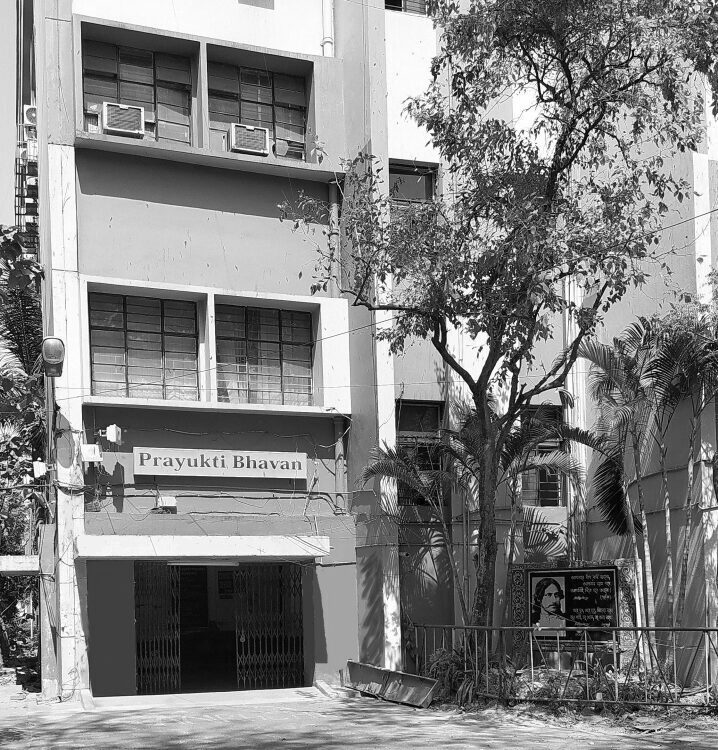
\includegraphics[width=0.3\linewidth]{images/prayukti.jpg}}
  \raisebox{-0.55\height}{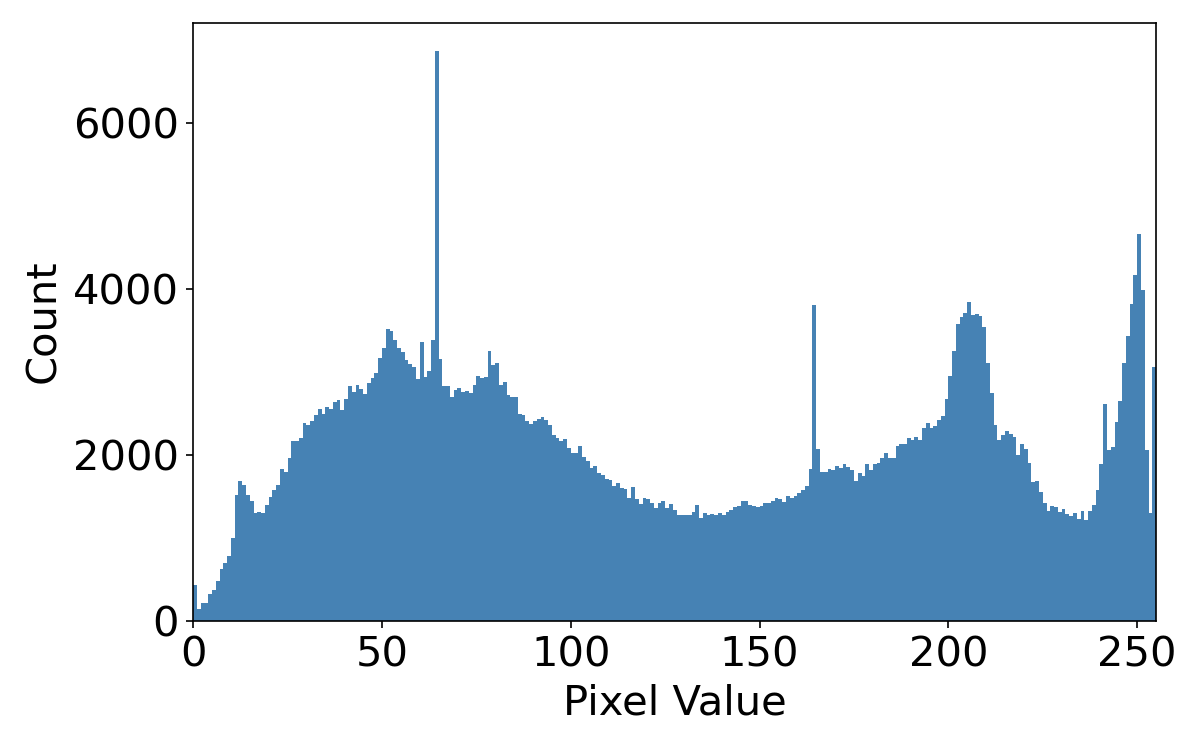
\includegraphics[width=0.6\linewidth]{images/prayukti_histogram.png}}
  \caption{Example image and its histogram}
\end{figure}

\subsection*{Contrast Stretching}

Contrast stretching (normalization) linearly expands an image’s
dynamic range, making low-contrast images more vivid. It’s the
simplest boost, though it can exaggerate noise or outliers.

\begin{equation*}
  s_k = T(r_k)
  = \frac{r_k - r_{\min}}{r_{\max} - r_{\min}}
  \times (L - 1)
\end{equation*}

where: (i) $r_k\rightarrow$ input intensity, (ii) $s_k\rightarrow$
output intensity, (iii) $r_{\min},\,r_{\max}\rightarrow$ observed
minimum and maximum intensities in the image, (iv) $L\rightarrow$
number of possible intensity levels

\begin{algorithm}[ht!]
  \DontPrintSemicolon
  Find $r_{\min}$ and $r_{\max}$ in input image $I$ \;
  {
    \ForEach{\textnormal{pixel intensity} $r_k \in I$}{
      $s_k \leftarrow \bigl(r_k -
      r_{\min}\bigr)\,/\,\bigl(r_{\max}-r_{\min}\bigr)\times(L-1)$ \;
      Clip $s_k$ to $[0,\,L-1]$ \;
    }
  }
  Return contrast-stretched image $I'$\;
  \caption{Contrast Stretching}
\end{algorithm}

\subsection*{Histogram Equalization}

Refers to \enquote{spreading out} (equalizing) the frequencies in an
image. Simple way to improve dark or washed out images.

\begin{equation*}
  s_k = T(r_k) = \sum_{j=1}^{k} p_r(r_j) = \sum_{j=1}^{k} \frac{n_j}{n}
\end{equation*}

where: (i) $r_k \rightarrow$ input intensity, (ii) $s_k \rightarrow$
processed intensity, (iii) $k \rightarrow$ intensity range (e.g. 0 -
1), (iv) $n_j \rightarrow$ frequency of intensity $j$, (v) $n
\rightarrow$ total number of pixels (v) $L\rightarrow$ number of
possible intensity levels

\begin{algorithm}[ht!]
  \DontPrintSemicolon
  Compute histogram of input image $I$ \;
  Compute CDF from histogram \;
  Normalize CDF by dividing by $n$ \;

  {
    Apply $T$ to each pixel intensity $r_k$ in $I$\\
    \nonl $s_k = \text{CDF}[r_k] \times (L - 1)$ \\
    \nonl where $L$ is the number of intensity levels \;
  }

  Return enhanced image $I'$\;
  \caption{Histogram Equalization}
\end{algorithm}

\subsection*{Point Processing}

Simplest spatial domain operation, neighborhood is the pixel itself.

\subsubsection*{Negative Images}

Simply inverts pixel values; useful for enhancing dark regions.
\begin{equation*}
  s = (L - 1) - r
\end{equation*}

\subsubsection*{Thresholding}

Segments an image by \textbf{converting it to binary} based on a
threshold value (say $\theta_0$); useful for isolating objects from
the background.

\begin{equation*}
  s =
  \begin{cases}
    0 & \text{if } r < \theta_0 \\
    L - 1 & \text{if } r \geq \theta_0
  \end{cases}
\end{equation*}

\subsubsection*{Gray Level Transforms}

\begin{figure}[H]
  \centering
  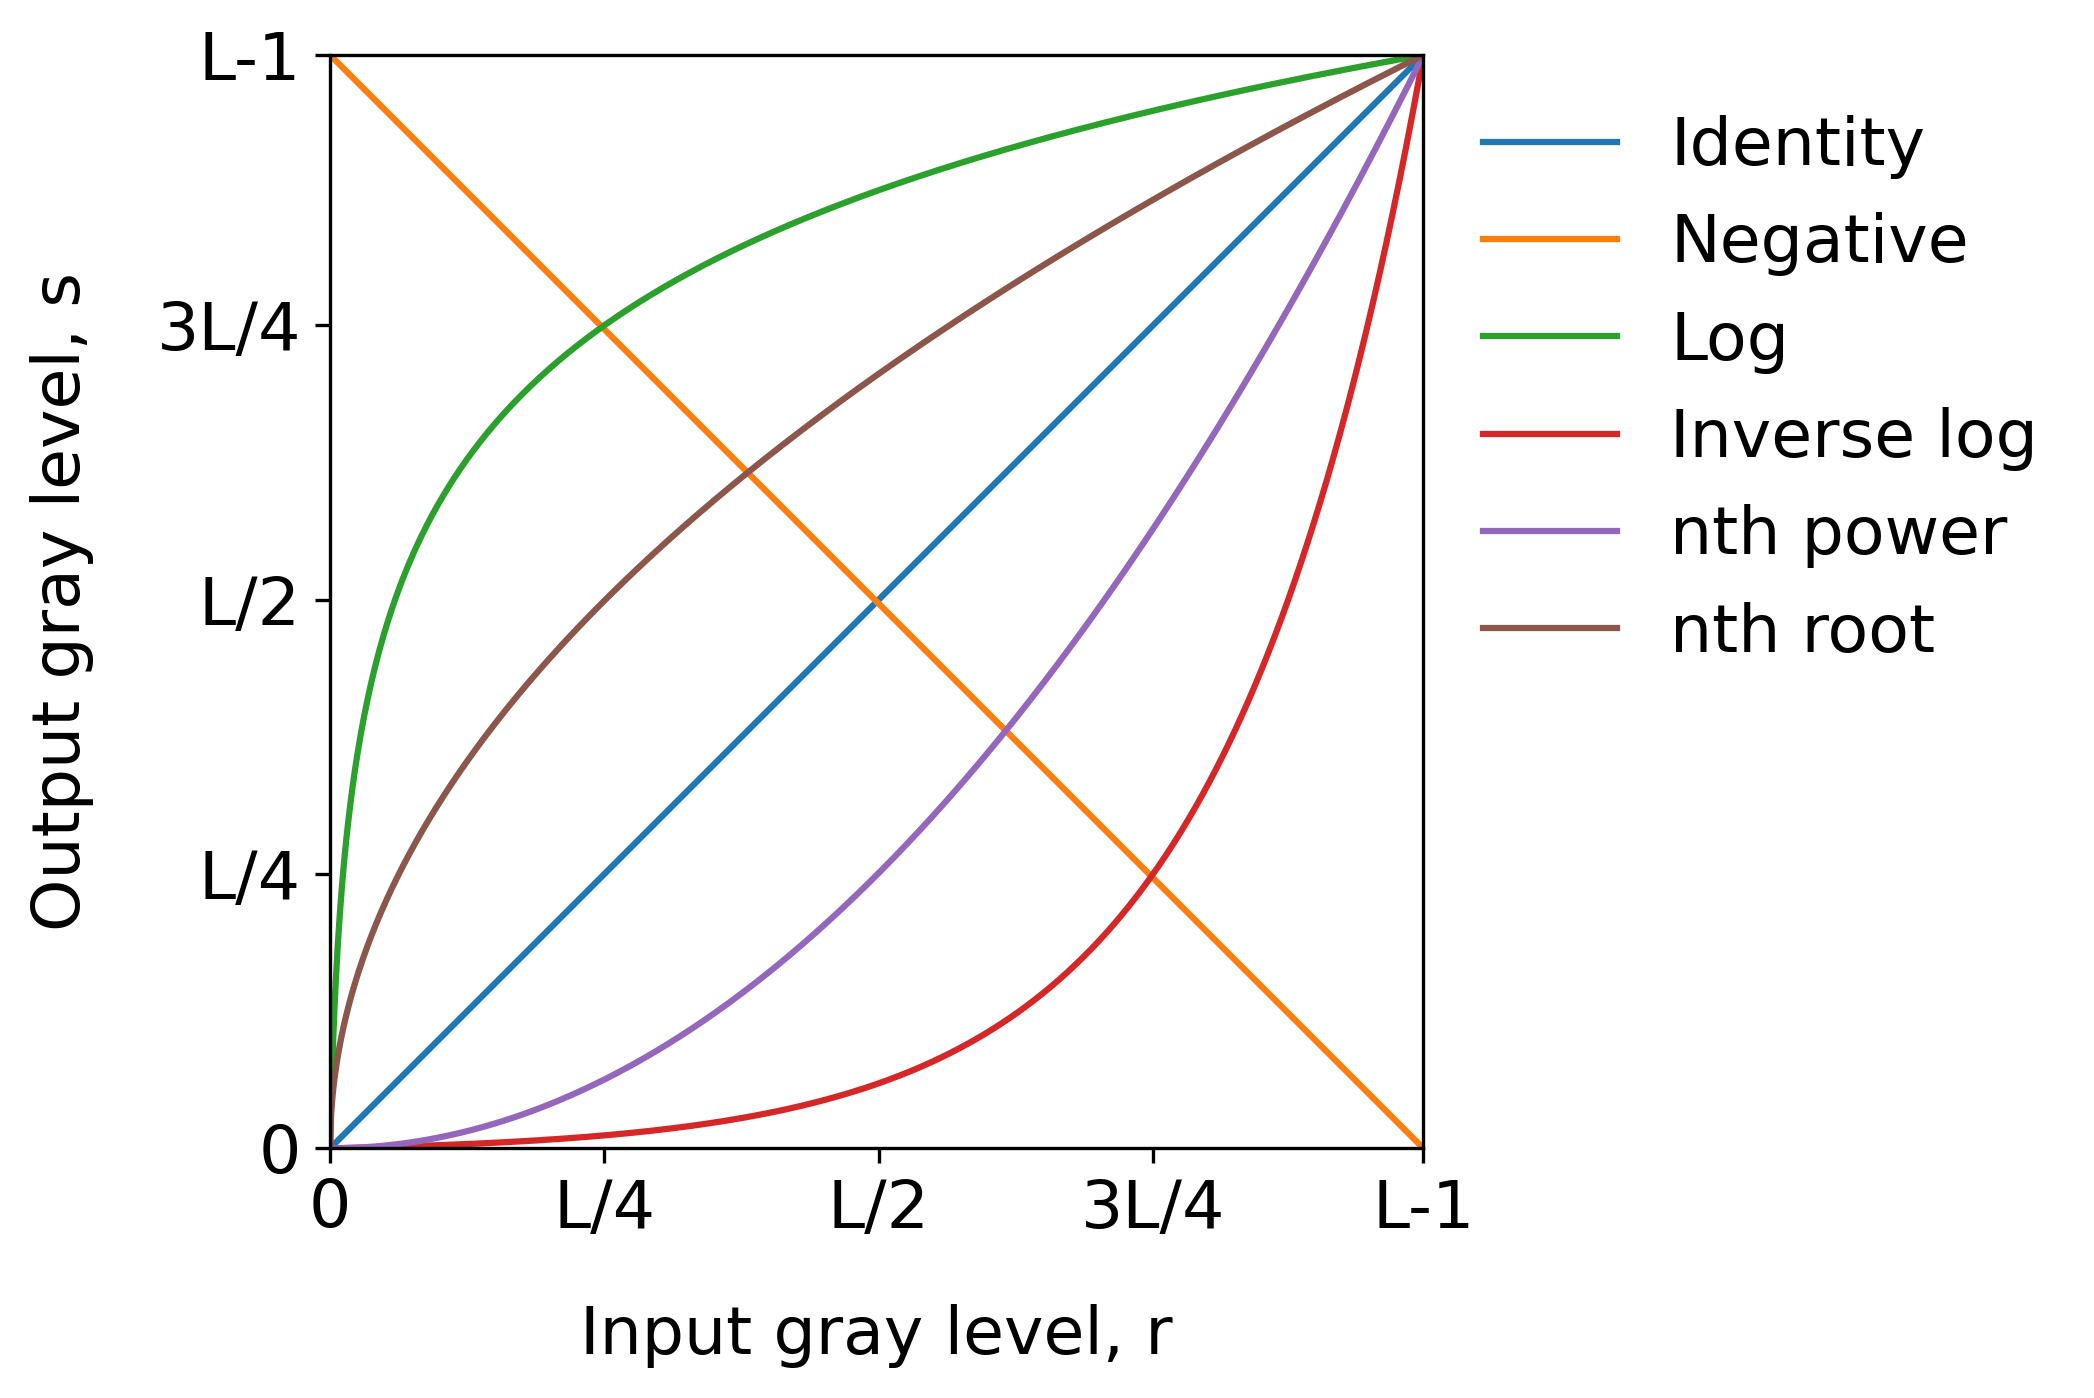
\includegraphics[width=\linewidth]{images/gray_level_transforms.png}
  \caption{Gray level transforms}
\end{figure}

\begin{itemize}
  \item \textbf{Log Transform:} Maps a narrow range of low input grey
    level values into a wider range of output values.
    \begin{itemize}
      \item $s = c \times \log(1 + r)$, where $c$ is a constant
      \item Useful when the input grey level values may have an
        extremely large range of values
      \item Use case 1: \textbf{log transform on Fourier transform}.
        More details are revealed.
      \item Use case 2: \textbf{gamma correction in displays}. Some
        displays do not respond linearly to different intensities;
        can be corrected using log transform
    \end{itemize}

  \item \textbf{Power Law Transform:} Maps a narrow range of dark
    input grey level values into a wider range of output values.
    \begin{itemize}
      \item $s = c \times r^{\gamma}$, where $\gamma$ is a constant
      \item Different $\gamma$ values highlight different details
      \item Useful for enhancing images with high dynamic range
    \end{itemize}

  \item \textbf{Piecewise Linear Transform:} Combines multiple
    arbitrary user-defined linear segments to create a more complex mapping.
    \begin{itemize}
      \item Useful for enhancing specific ranges of pixel values
      \item Can be used to adjust contrast in specific regions of an image
    \end{itemize}

    \begin{minipage}{\linewidth}
      \vspace{-0.5cm}
      \begin{figure}[H]
        \centering
        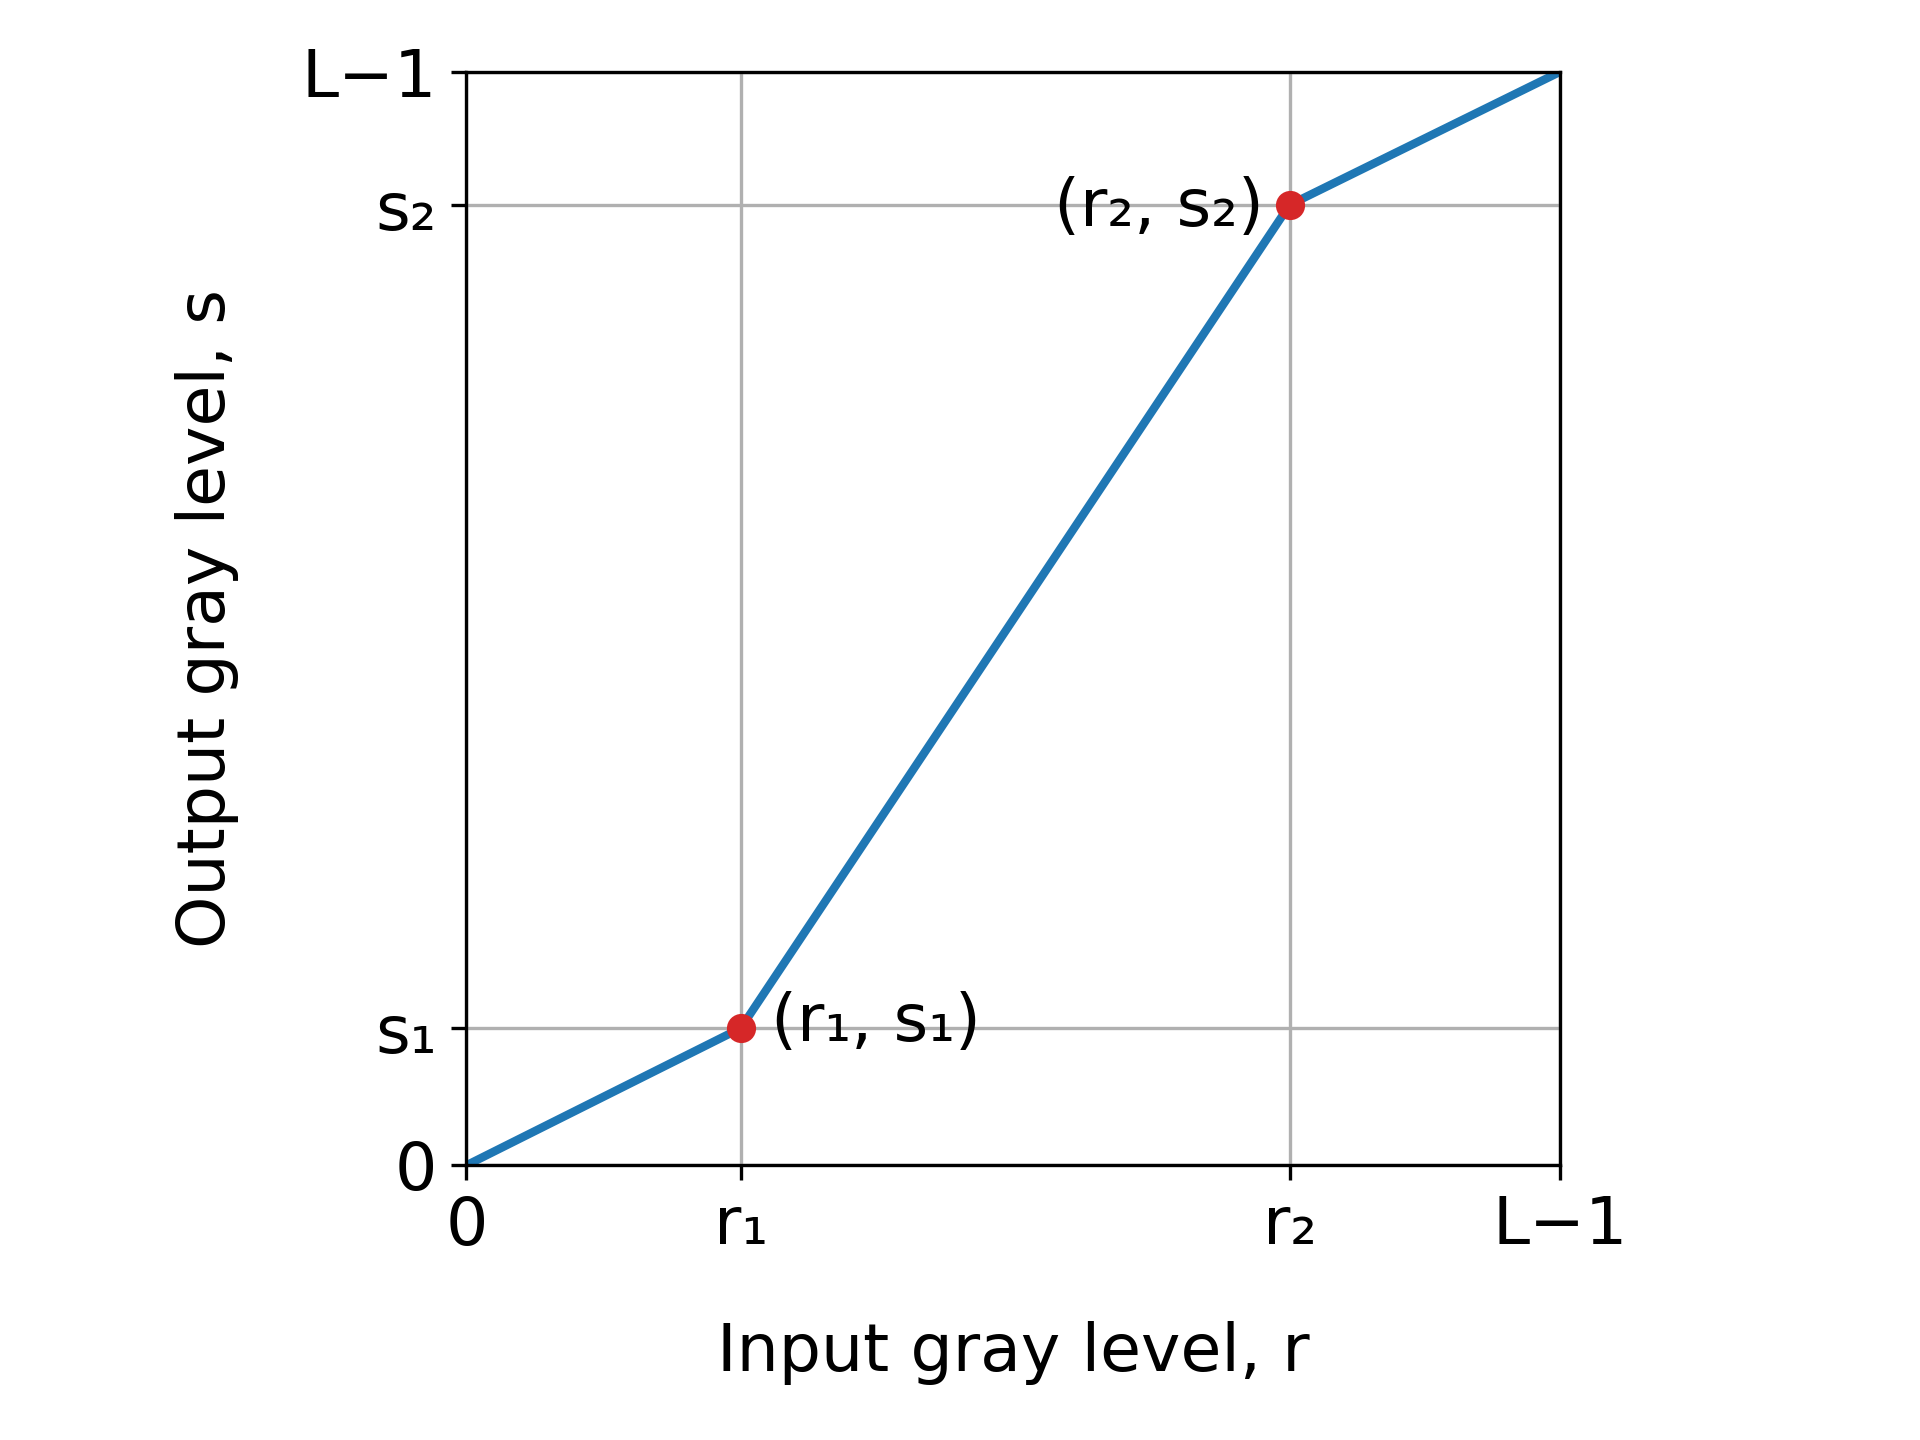
\includegraphics[width=\linewidth]{images/piecewise_transform.png}
        \vspace{-0.5cm}
        \caption{Piecewise linear transform}
      \end{figure}
    \end{minipage}

  \item \textbf{Gray Level Slicing:} Similar to thresholding, but
    allows for a range of pixel values to be highlighted.
    \begin{itemize}
      \item Other levels can be suppressed or maintained
      \item Useful for enhancing specific features in an image
    \end{itemize}

    \begin{minipage}{\linewidth}
      \begin{figure}[H]
        \centering
        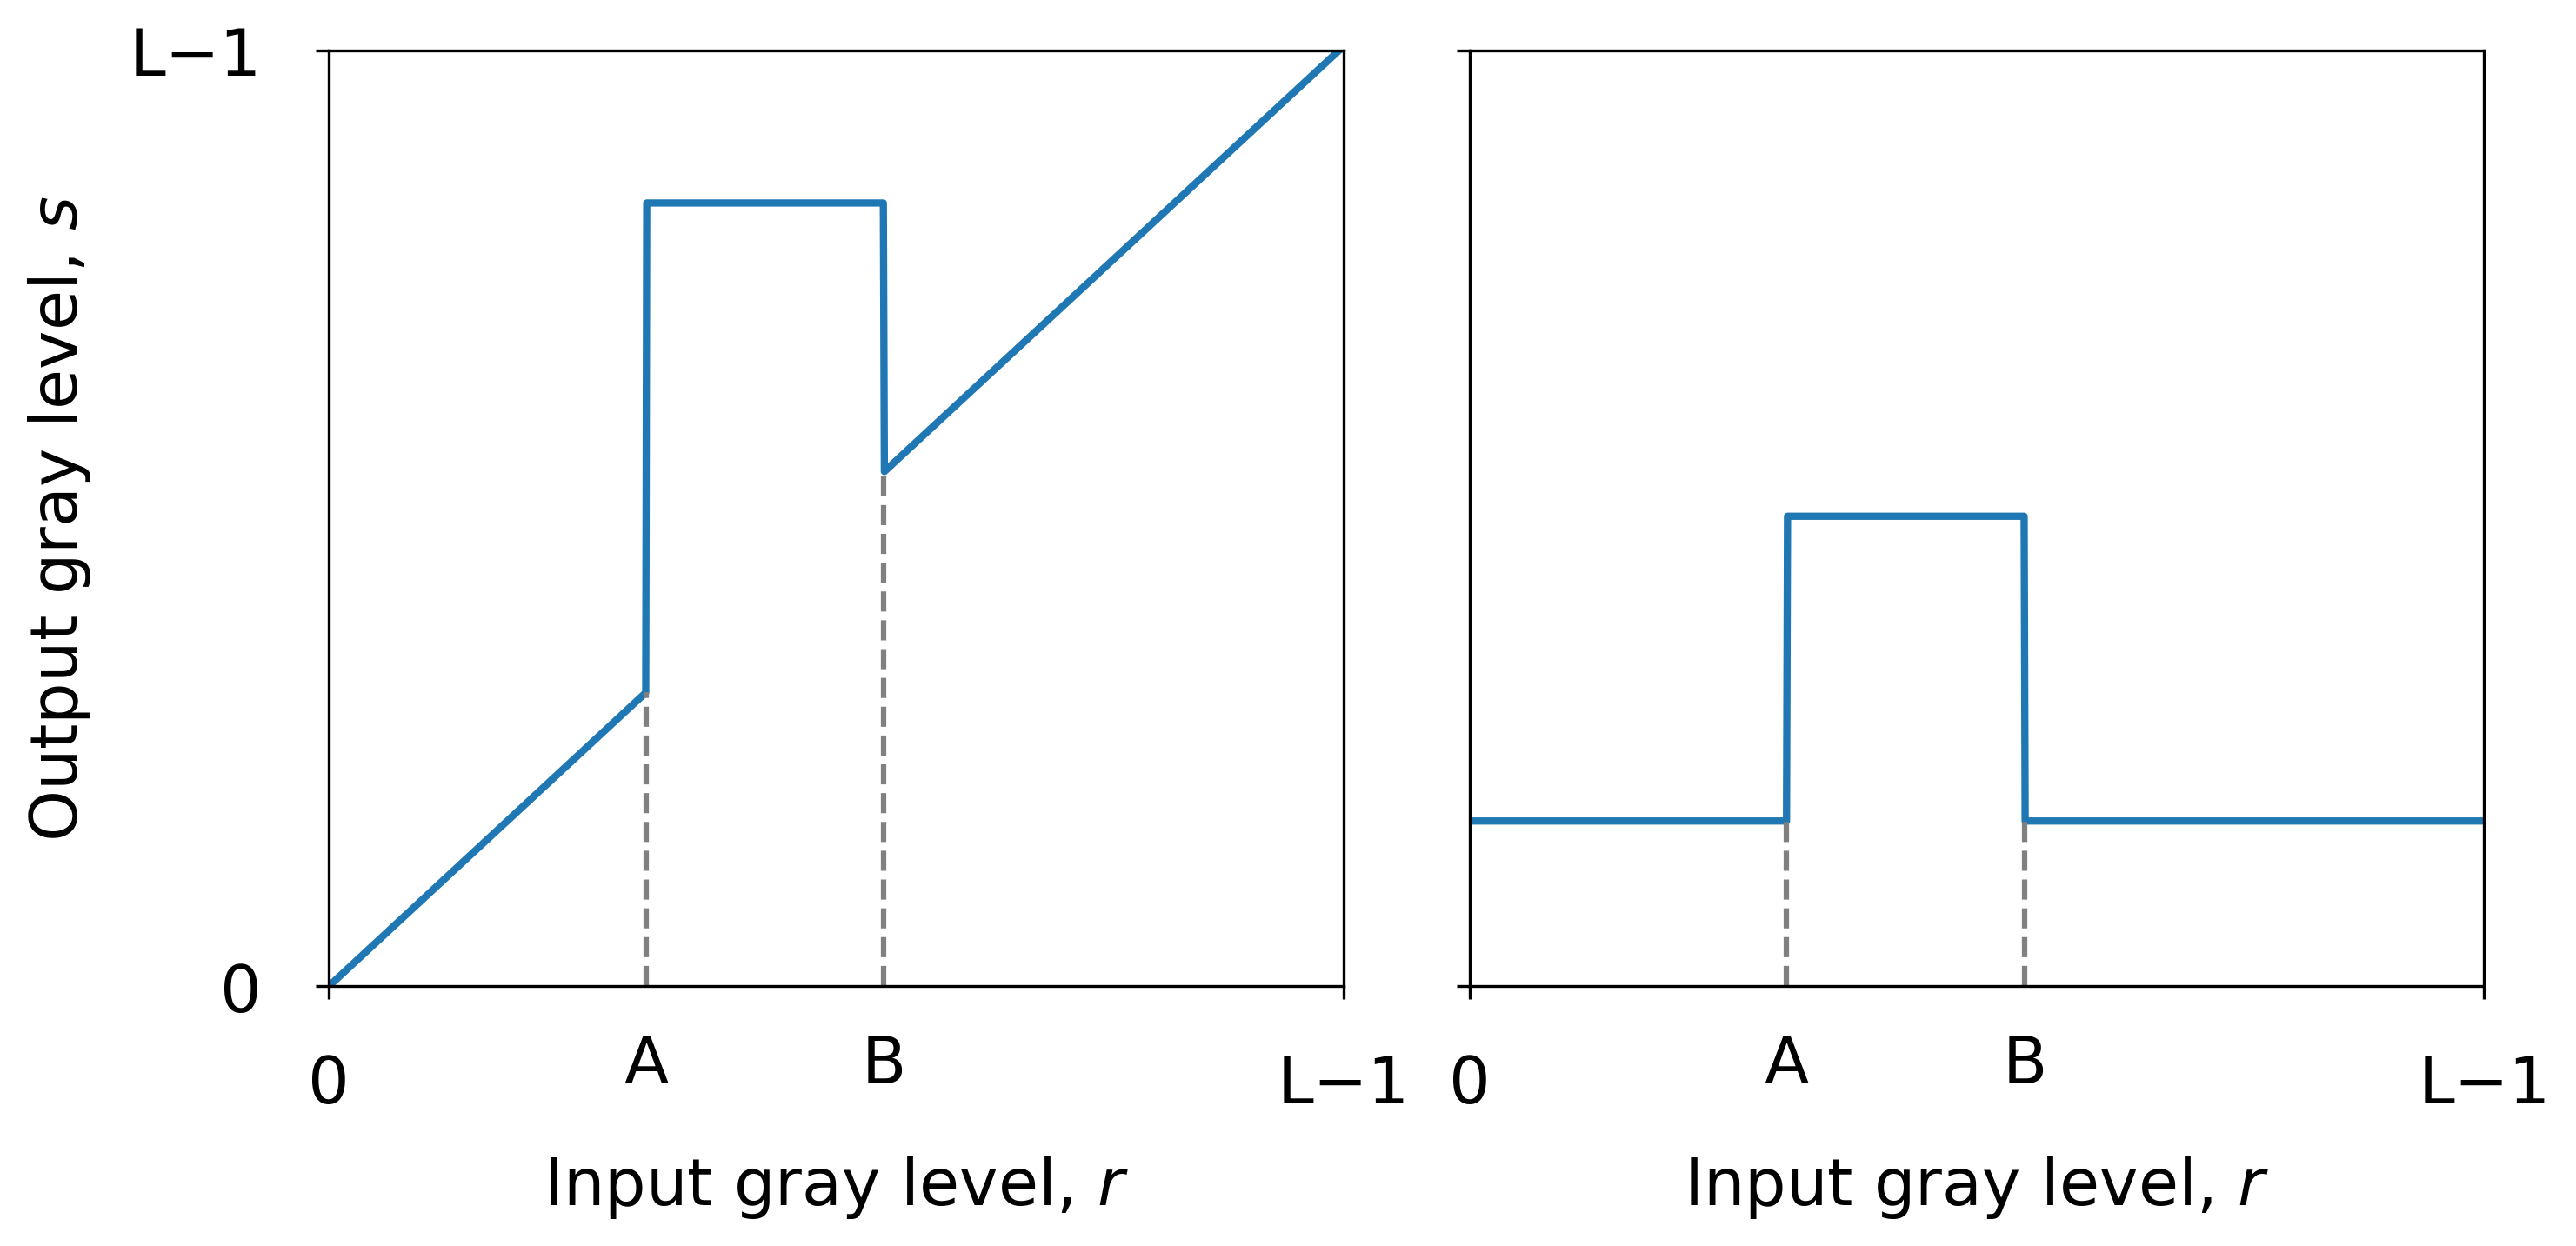
\includegraphics[width=\linewidth]{images/gray_level_slicing.png}
        \caption{Gray level slicing with (i) background retained (ii)
        background supressed}
      \end{figure}
    \end{minipage}

  \item \textbf{Bit-Plane Slicing:} By isolating particular bits of
    the pixel values in an image, we can highligh interesting aspects
    of that image.
    \begin{itemize}
      \item Higher order bits contain most of the significant information
      \item Lower order bits contain subtle details
      \item \enquote{Bit planes} are arranged in a stack; MSB at the
        top, LSB at the bottom.
    \end{itemize}

    \begin{minipage}{\linewidth}
      \begin{figure}[H]
        \centering
        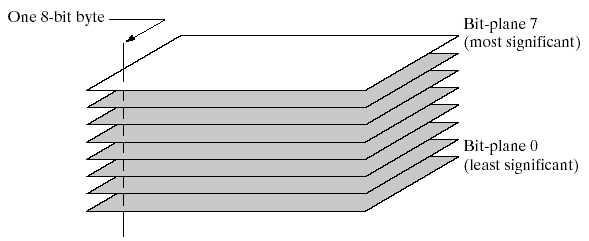
\includegraphics[width=\linewidth]{images/bit_plane_slicing.png}
        \caption{Bit-plane slicing of an 8-bit image}
      \end{figure}
      \vspace{-0.5cm}
    \end{minipage}

\end{itemize}

\subsection*{Neighborhood Operations}

Operations on a \textbf{rectangular region} around a pixel. Any size
rectangle and any shape filter are possible.

\subsubsection*{Simple Neighborhood Operations}

For any pixel $p$ in an image at the center of a neighborhood:

\begin{itemize}
  \item \textbf{Min:} Sets $p$ to minimum value in the neighborhood.
    \begin{itemize}
      \item Removes small bright spots (\textbf{salt noise})
      \item Makes \textbf{dark regions darker}
    \end{itemize}
  \item \textbf{Max:} Sets $p$ to maximum value in the neighborhood.
    \begin{itemize}
      \item Removes small dark spots (\textbf{pepper noise})
      \item Makes \textbf{bright regions brighter}
    \end{itemize}
  \item \textbf{Median:} Sets $p$ to median value in the neighborhood.
    \begin{itemize}
      \item Removes \textbf{salt and pepper noise}
    \end{itemize}
\end{itemize}

\subsubsection*{Correlation vs Convolution}

Most spatial filtering operations are technically
\textbf{correlation}, and the filter is referred to as a
\textbf{correlation kernel} or \textbf{mask}. \textbf{Convolution} is
a similar operation, with a subtle difference:

\begin{figure}[H]
  \centering
  \begin{tikzpicture}[%
      imgcell/.style={draw=black, fill=white, minimum size=1cm, anchor=center},
      filtercell/.style={draw=MaterialBlue900, fill=MaterialBlue50,
      minimum size=1cm, anchor=center}
    ]

    % Original image grid
    \node[imgcell] (i11) at (0,2) {$r_1$};
    \node[imgcell] (i12) at (1,2) {$r_2$};
    \node[imgcell] (i13) at (2,2) {$r_3$};
    \node[imgcell] (i21) at (0,1) {$r_4$};
    \node[imgcell, fill=MaterialGrey200] (i22) at (1,1) {$r_5$};
    \node[imgcell] (i23) at (2,1) {$r_6$};
    \node[imgcell] (i31) at (0,0) {$r_7$};
    \node[imgcell] (i32) at (1,0) {$r_8$};
    \node[imgcell] (i33) at (2,0) {$r_9$};

    % Convolution symbol
    \node at (3,1) {\large $\ast$};

    % Filter grid
    \node[filtercell] (f11) at (4,2) {$k_1$};
    \node[filtercell] (f12) at (5,2) {$k_2$};
    \node[filtercell] (f13) at (6,2) {$k_3$};
    \node[filtercell] (f21) at (4,1) {$k_4$};
    \node[filtercell] (f22) at (5,1) {$k_5$};
    \node[filtercell] (f23) at (6,1) {$k_6$};
    \node[filtercell] (f31) at (4,0) {$k_7$};
    \node[filtercell] (f32) at (5,0) {$k_8$};
    \node[filtercell] (f33) at (6,0) {$k_9$};

  \end{tikzpicture}
  \caption{An image (left) being operated on by a filter (right). The
    result depends
  on whether the operation is correlation or convolution.}
\end{figure}
\vspace{-0.5cm}
\begin{itemize}
  \item \textbf{Correlation:} The filter is applied directly to the
    image, without flipping it.
    \vspace{-0.2cm}
    \begin{equation*}
      s = r_1 k_1 + r_2 k_2 + r_3 k_3 + r_4 k_4 + r_5 k_5 + r_6 k_6 +
      r_7 k_7 + r_8 k_8 + r_9 k_9\\[-0.3cm]
    \end{equation*}
  \item \textbf{Convolution:} The filter is flipped both horizontally
    and vertically before being applied to the image.
    \vspace{-0.2cm}
    \begin{equation*}
      s = r_1 k_9 + r_2 k_8 + r_3 k_7 + r_4 k_6 + r_5 k_5 + r_6 k_4 +
      r_7 k_3 + r_8 k_2 + r_9 k_1
    \end{equation*}
\end{itemize}

\subsubsection*{Linear Spatial Filters}

\begin{equation*}
  g(x, y) = \sum_{s=-a}^{a} \sum_{t=-b}^{b} w(s, t) f(x + s, y + t)
\end{equation*}

\begin{itemize}
  \item \textbf{Smoothing Filters:} Smooths an image by averaging
    pixel values in the neighborhood.
    \begin{itemize}
      \item Simplest form: \textbf{mean filter} or \textbf{simple
        averaging filter}; $k \times k$ matrix, each
        element is $1/k^2$.

        \begin{minipage}{\linewidth}
          \vspace{-0.3cm}
          \begin{figure}[H]
            \centering
            \begin{tikzpicture}[%
                filtercell/.style={draw=MaterialBlue900, fill=MaterialBlue50,
                minimum size=1cm, anchor=center}
              ]
              \node[filtercell] (f11) at (0,2) {$1/9$};
              \node[filtercell] (f12) at (1,2) {$1/9$};
              \node[filtercell] (f13) at (2,2) {$1/9$};
              \node[filtercell] (f21) at (0,1) {$1/9$};
              \node[filtercell] (f22) at (1,1) {$1/9$};
              \node[filtercell] (f23) at (2,1) {$1/9$};
              \node[filtercell] (f31) at (0,0) {$1/9$};
              \node[filtercell] (f32) at (1,0) {$1/9$};
              \node[filtercell] (f33) at (2,0) {$1/9$};

            \end{tikzpicture}
            \caption{Simple 3x3 averaging filter}
          \end{figure}
        \end{minipage}
      \item Sometimes different pixels in the neighborhood are
        weighted differently (\textbf{weighted averaging filter}).
        The filter values always add up to 1.

        \begin{minipage}{\linewidth}
          \vspace{-0.3cm}
          \begin{figure}[H]
            \centering
            \begin{tikzpicture}[%
                filtercell/.style={draw=MaterialBlue900, fill=MaterialBlue50,
                minimum size=1cm, anchor=center}
              ]
              \node[filtercell] (f11) at (0,2) {$1/16$};
              \node[filtercell] (f12) at (1,2) {$2/16$};
              \node[filtercell] (f13) at (2,2) {$1/16$};
              \node[filtercell] (f21) at (0,1) {$2/16$};
              \node[filtercell] (f22) at (1,1) {$4/16$};
              \node[filtercell] (f23) at (2,1) {$2/16$};
              \node[filtercell] (f31) at (0,0) {$1/16$};
              \node[filtercell] (f32) at (1,0) {$2/16$};
              \node[filtercell] (f33) at (2,0) {$1/16$};

            \end{tikzpicture}
            \caption{Weighted 3x3 averaging filter}
          \end{figure}
        \end{minipage}

      \item \textbf{Useful for}: (i) removing noise from images (ii)
        highlighting gross details
    \end{itemize}
  \item \textbf{Sharpening Filters:} Enhances edges and fine
    details in an image.
    \begin{itemize}
      \item \textbf{Laplacian Filter:} Highlights regions of rapid
        intensity change (edges and other discontinuities).

        \begin{minipage}{\linewidth}
          \vspace{-0.3cm}
          \begin{figure}[H]
            \centering
            \begin{tikzpicture}[%
                filtercell/.style={draw=MaterialBlue900, fill=MaterialBlue50,
                minimum size=1cm, anchor=center}
              ]
              \node[filtercell] (f111) at (0,2) {$0$};
              \node[filtercell] (f112) at (1,2) {$-1$};
              \node[filtercell] (f113) at (2,2) {$0$};
              \node[filtercell] (f121) at (0,1) {$-1$};
              \node[filtercell] (f122) at (1,1) {$4$};
              \node[filtercell] (f123) at (2,1) {$-1$};
              \node[filtercell] (f131) at (0,0) {$0$};
              \node[filtercell] (f132) at (1,0) {$-1$};
              \node[filtercell] (f133) at (2,0) {$0$};

              \node[filtercell] (f211) at (4,2) {$0$};
              \node[filtercell] (f212) at (5,2) {$-1$};
              \node[filtercell] (f213) at (6,2) {$0$};
              \node[filtercell] (f221) at (4,1) {$-1$};
              \node[filtercell] (f222) at (5,1) {$5$};
              \node[filtercell] (f223) at (6,1) {$-1$};
              \node[filtercell] (f231) at (4,0) {$0$};
              \node[filtercell] (f232) at (5,0) {$-1$};
              \node[filtercell] (f233) at (6,0) {$0$};

            \end{tikzpicture}
            \caption{Laplacian filter (left), filter which yields
            Laplacian result subtracted from original image (right)}

          \end{figure}
        \end{minipage}

    \end{itemize}
\end{itemize}
